\documentclass[]{article}
\newcommand{\FileDepth}{../../..}
\usepackage[letterpaper, landscape, margin=0.5cm]{geometry}
\usepackage[T1]{fontenc}
\usepackage{textcomp}%Not strictly necessary, but gives \textmu command for "micro."
\usepackage{fancyhdr}
\usepackage{amsmath}
\usepackage{amssymb}
\usepackage{graphicx}
\usepackage{xcolor}
\usepackage{tikz}
\usetikzlibrary{calc}
\usepackage[shortlabels]{enumitem}
\usepackage{multicol}
\usepackage{vwcol}
\usepackage{hyperref}
\usepackage{wrapfig}
%opening
\newcommand{\SecType}{L}
\newcommand{\Week}{8}
\title{PH 211 Lecture \Week}
\author{Benjamin Bauml}
\date{Summer 2024}

\newcommand{\Purpose}{4}
\newcommand{\DefOnly}{0}

\input{\FileDepth/Formats/Assignment20240614.tex}
\usepackage[absolute]{textpos}
% This package relies on Assignment Format 2024-06-14 or later to work. It is recommended that the Purpose and DefOnly commands be given as such:
%\newcommand{\Purpose}{4}
%\newcommand{\DefOnly}{0}
% Activities need to be entered outside of the TeacherMargin and PresentSpace environments, otherwise they will be defined only locally. They can even go in the preamble.
\newenvironment{TeacherMargin}{\begin{textblock*}{10.8cm}(0.5cm,0.5cm)
\small}{\end{textblock*}
\hspace{0.1cm}}
\newenvironment{PresentSpace}{\begin{textblock*}{0.3cm}(26.85cm,9.35cm)
--
\end{textblock*}
\begin{textblock*}{15.6cm}(11.8cm,0.5cm)
\begin{Repurpose}{1}
\Large}{\end{Repurpose}
\end{textblock*}
\hspace{0.1cm}}

\newcommand{\FBDaxes}[4][2]{
	\begin{scope}[shift={(#2)},rotate=#3]
		% x-axis
		\draw[thick,->] (-#1,0) -- (#1,0);
		\node[anchor=west] at (#1,0) {$x$};
		% y-axis
		\draw[thick,->] (0,-#1) -- (0,#1);
		\node[anchor=south] at (0,#1) {$y$};
		\coordinate (#4) at (0,0);
	\end{scope}
}
\newcommand{\FBDvectorMA}[4]{
	\begin{scope}[shift={(#1)}]
		\coordinate (#4tip) at ({#2*cos(#3)},{#2*sin(#3)});
		\draw[ultra thick,blue,->] (#1) -- (#4tip);
	\end{scope}
}
\newcommand{\FBDvectorXY}[3]{
	\begin{scope}[shift={(#1)}]
		\coordinate (#3tip) at (#2);
		\draw[ultra thick,blue,->] (0,0) -- (#3tip);
	\end{scope}
}
\newcommand{\FBDdot}[1]{
	\filldraw[black] (#1) circle (3pt);
}
\newcommand{\FBDbox}[5][1]{
	\begin{scope}[shift={(#2)},rotate=#3]
		\filldraw[color=black,fill=white,thick] ({-#1/2},{#1/2}) -- ({-#1/2},{-#1/2}) -- ({#1/2},{-#1/2}) -- ({#1/2},{#1/2}) -- cycle;
		% Left side coordinates
		\coordinate (#4ltq) at ({-#1/2},{#1/4});
		\coordinate (#4lcent) at ({-#1/2},0);
		\coordinate (#4lbq) at ({-#1/2},{-#1/4});
		% right side coordinates
		\coordinate (#4rtq) at ({#1/2},{#1/4});
		\coordinate (#4rcent) at ({#1/2},0);
		\coordinate (#4rbq) at ({#1/2},{-#1/4});
		% top coordinates
		\coordinate (#4tlq) at ({-#1/4},{#1/2});
		\coordinate (#4tcent) at (0,{#1/2});
		\coordinate (#4trq) at ({#1/4},{#1/2});
		% bottom coordinates
		\coordinate (#4blq) at ({-#1/4},{-#1/2});
		\coordinate (#4bcent) at (0,{-#1/2});
		\coordinate (#4brq) at ({#1/4},{-#1/2});
		% corners
		\coordinate (#4tl) at ({-#1/2},{#1/2});
		\coordinate (#4tr) at ({#1/2},{#1/2});
		\coordinate (#4bl) at ({-#1/2},{-#1/2});
		\coordinate (#4br) at ({#1/2},{-#1/2});
		\node at (0,0) {#5};
	\end{scope}
}
%\newcommand{\MVec}[3][0]{%Creates a momentum vector of length #3 centered at #2 and rotated #1 degrees counterclockwise.
	\begin{scope}[rotate=#1,shift={(#2)}]
		\draw[->,thick] ({-#3/2},0) -- ({#3/2},0);
	\end{scope}
}
\newcommand{\MDot}[1]{%Creates a dot at #1 to represent a zero vector.
	\filldraw (#1) circle (1pt);
}
\newcommand{\MVDRows}[2][4.5]{%Creates the rows (initial, delta, final) of a momentum vector diagram. The optional argument determines the width of the table, and defaults to a good length for three columns (two objects and the total system). The non-optional argument gives a coordinate name (not displayed) to the diagram.
	\begin{scope}
		%\draw[thick] (0,5.5) -- (0,0);
		\draw[thick] (-1,4.5) -- (#1,4.5);
		\node at (-0.5,3.75) {$\vec{p}_{i}$};
		\draw[thick] (-1,3) -- (#1,3);
		\node at (-0.5,2.25) {$\Delta\vec{p}$};
		\draw[thick] (-1,1.5) -- (#1,1.5);
		\node at (-0.5,0.75) {$\vec{p}_{f}$};
		\coordinate (#2) at (0,5);
	\end{scope}
}
\newcommand{\MVDCol}[4][0.75]{%Creates a column for an object in a momentum vector diagram. The first (non-optional) argument is the coordinate name (not displayed) of the column, while the second is the displayed column header. The first argument also names the three entries down the column. The third argument anchors the column, so it should either be the coordinate name of the MVD (for the first column) or the coordinate name of the previous column. The optional argument indicates how far the center of the column should be from the previous column's edge, and defaults to 0.75.
	\begin{scope}[shift={(#4)}]
		\node at (#1,0) {#3};
		%\draw[thick] ({#1*2},0.5) -- ({#1*2},-5);
		\draw[thick] (0,0.5) -- (0,-5);
		\coordinate (#2init) at (#1,-1.25);
		\coordinate (#2delt) at (#1,-2.75);
		\coordinate (#2fin) at (#1,-4.25);
		\coordinate (#2) at ({#1*2},0);
	\end{scope}
}

%\input{\FileDepth/Activities/Activity_One/Activity_One.tex}
%\input{\FileDepth/Activities/Activity_Two/Activity_Two.tex}

\begin{document}
\begin{TeacherMargin}
\noindent Friction is always parallel to the surface of contact, so (C) and (G) are the only possible answers. If we pick (G) and look at the free-body diagram,
\begin{center}
	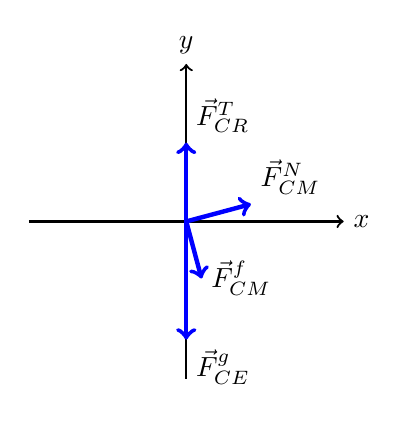
\begin{tikzpicture}
		\FBDaxes{0,0}{0}{axes}
		\FBDvectorXY{0,0}{0,-1.5}{FG}
		\node[anchor=north west] at (FGtip) {$\vec{F}^{g}_{CE}$};
		\FBDvectorXY{0,0}{0,1}{FT}
		\node[anchor=south west] at (FTtip) {$\vec{F}^{T}_{CR}$};
		\FBDvectorMA{0,0}{0.85}{15}{FN}
		\node[anchor=south west] at (FNtip) {$\vec{F}^{N}_{CM}$};
		\FBDvectorMA{0,0}{0.75}{-75}{FF}
		\node[anchor=west] at (FFtip) {$\vec{F}^{f}_{CM}$};
	\end{tikzpicture}
\end{center}
we find that the $x$-component of the net force is positive, which would make the climber accelerate. We need friction to go in direction (C) if we want to balance the forces in the $x$-direction.
\begin{center}
	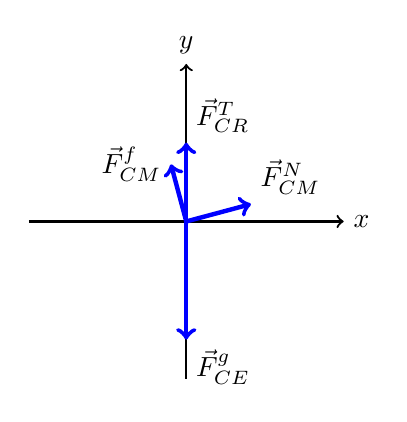
\begin{tikzpicture}
		\FBDaxes{0,0}{0}{axes}
		\FBDvectorXY{axes}{0,-1.5}{FG}
		\node[anchor=north west] at (FGtip) {$\vec{F}^{g}_{CE}$};
		\FBDvectorXY{axes}{0,1}{FT}
		\node[anchor=south west] at (FTtip) {$\vec{F}^{T}_{CR}$};
		\FBDvectorMA{axes}{0.85}{15}{FN}
		\node[anchor=south west] at (FNtip) {$\vec{F}^{N}_{CM}$};
		\FBDvectorMA{axes}{0.75}{105}{FF}
		\node[anchor=east] at (FFtip) {$\vec{F}^{f}_{CM}$};
	\end{tikzpicture}
\end{center}
This FBD is out of scale, as the $y$-components of the tension, normal force, and friction clearly add to be larger than the force of gravity, and we need the $x$-components of friction and the normal force to be equal in magnitude to cancel out.
\end{TeacherMargin}
\begin{PresentSpace}
\begin{center}
	\huge Lecture 8: Free-Body Diagrams
\end{center}
\vspace{0.5cm}
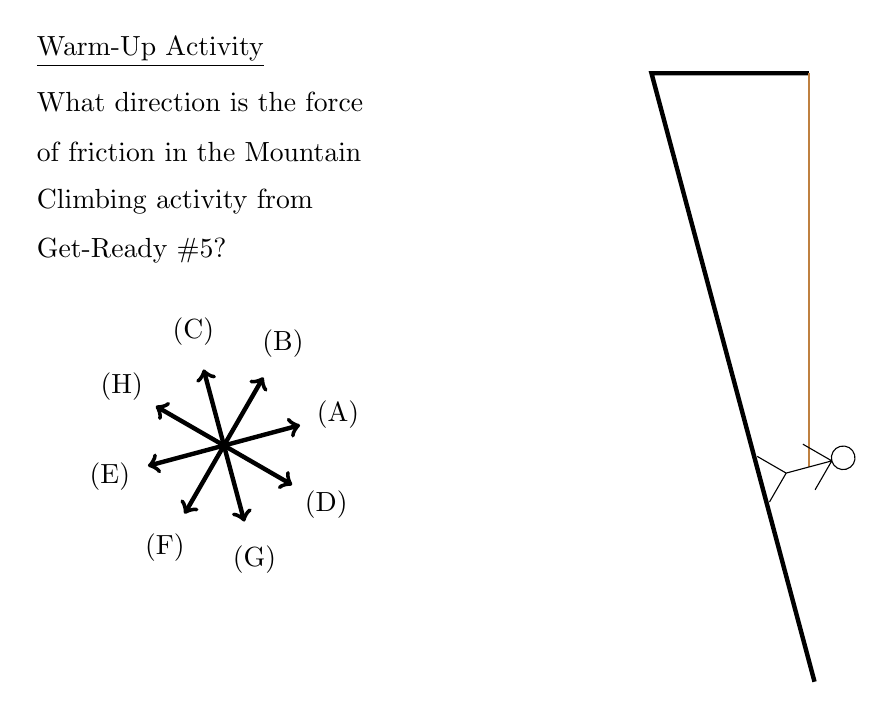
\begin{tikzpicture}
	\node[anchor=west] at (0,0) {\underline{Warm-Up Activity}};
	\node[anchor=west] at (0,-18pt) {What direction is the force};
	\node[anchor=west] at (0,-36pt) {of friction in the Mountain};
	\node[anchor=west] at (0,-54pt) {Climbing activity from};
	\node[anchor=west] at (0,-72pt) {Get-Ready \#5?};
	\foreach \th in {0,45,90,135}
		\draw[ultra thick,<->,shift={(2.5,-5)},rotate={\th-75}] (-1,0) -- (1,0);
	\foreach \th in {0,45,90,135}
		\coordinate[shift={(2.5,-5)}] (ArL\th) at ({-1.5*cos(\th+75)},{1.5*sin(\th+75)});
	\foreach \th in {0,45,90,135}
		\coordinate[shift={(2.5,-5)}] (ArR\th) at ({1.5*cos(\th+75)},{-1.5*sin(\th+75)});
	\node at (ArL0) {(C)};
	\node at (ArR0) {(G)};
	\node at (ArL45) {(B)};
	\node at (ArR45) {(F)};
	\node at (ArL90) {(A)};
	\node at (ArR90) {(E)};
	\node at (ArL135) {(D)};
	\node at (ArR135) {(H)};
	\begin{scope}[shift={(10,-8)}]
		\draw[ultra thick] (0,0) -- ({-8*cos(75)},{8*sin(75)}) -- ({2-8*cos(75)},{8*sin(75)});
		\draw[thick,brown] ({2-8*cos(75)},{8*sin(75)}) -- ({2-8*cos(75)},{8*sin(75)-5});
	\end{scope}
	\begin{scope}[shift={({12-8*cos(75)},{8*sin(75)-13})},rotate=-75,scale=0.6]
		\draw (-0.5,-1) -- (0,-0.5) -- (0.5,-1) (0,-0.5) -- (0,0.5) (-0.5,0) -- (0,0.5) -- (0.5,0) (0,0.75) circle (0.25);
	\end{scope}
\end{tikzpicture}
\end{PresentSpace}
\newpage
\begin{TeacherMargin}

\end{TeacherMargin}
\begin{PresentSpace}
\vspace{-10pt}
\section*{Free-Body Diagrams and Systems}
\vspace{-10pt}
\begin{itemize}
	\item Choose a system.
	\begin{itemize}
		\large
		\item Make sure you know what is internal to your system and what is external to your system.
	\end{itemize}
	\item Identify and describe each external force:
	\begin{itemize}
		\large
		\item Say what kind of force it is.
		\item Determine the object the force is being acted on.
		\item Determine the object that is exerting the force.
		\item Write a symbolic version of the force that includes the information above.
		\item Represent all the forces acting on a single object or system using a \\
		\textbf{\underline{free-body diagram}}.
		\begin{itemize}
			\item All forces on the same free body diagram should act on the same thing (same first subscript).
		\end{itemize}
	\end{itemize}
\end{itemize}
\end{PresentSpace}
\begin{textblock*}{5cm}(22cm,3.5cm)
	\Huge
	\[
	\vec{F}^{\text{\Large\ type}}_{\text{\Large on,by}}
	\]
\end{textblock*}
\newpage
\begin{TeacherMargin}

\end{TeacherMargin}
\begin{PresentSpace}
\vspace{-10pt}
\section*{(Newton's) Laws of Motion}
\vspace{-10pt}
\begin{enumerate}[(1)]
	\item An object in motion (or at rest) stays in motion (or at rest) unless a net external force acts on it.
	\item The net force on an object is equal to the object's mass times its acceleration.
	\[
	\vec{F}^{net} = m\vec{a}
	\]
\end{enumerate}
\end{PresentSpace}
\newpage
\begin{TeacherMargin}
\noindent\textbf{Idenfity All Forces}
\begin{itemize}
	\item Mike is pushing directly into the side of the box, so we need a normal force on the box by Mike: $\vec{F}^{N}_{BM}$.
	\item The box has mass, so we need a force of gravity on the box from Earth: $\vec{F}^{g}_{BE}$.
	\item The rope held by Lucas is pulling on the box (Lucas himself is not directly touching it), so we need a force of tension on the box by the rope: $\vec{F}^{T}_{BR}$.
	\item The box is sitting on the ground and not budging, so we need a normal force on the box from the ground, and a force of static friction on the box from the ground: $\vec{F}^{N}_{BG}$ and $\vec{F}^{sf}_{BG}$.
\end{itemize}
\noindent\textbf{Free-Body Diagram}
\vspace{-0.75cm}
\begin{center}
	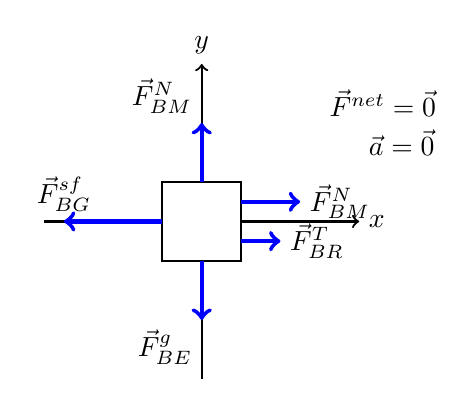
\begin{tikzpicture}
		\FBDaxes{0,0}{0}{axes}
		\FBDbox{axes}{0}{box}{}
		\FBDvectorXY{boxrtq}{0.75,0}{FNM}
		\node[anchor=west] at (FNMtip) {$\vec{F}^{N}_{BM}$};
		\FBDvectorXY{boxrbq}{0.5,0}{FTR}
		\node[anchor=west] at (FTRtip) {$\vec{F}^{T}_{BR}$};
		\FBDvectorXY{boxlcent}{-1.25,0}{FSF}
		\node[anchor=south] at (FSFtip) {$\vec{F}^{sf}_{BG}$};
		\FBDvectorXY{boxtcent}{0,0.75}{FNG}
		\node[anchor=south east] at (FNGtip) {$\vec{F}^{N}_{BM}$};
		\FBDvectorXY{boxbcent}{0,-0.75}{FG}
		\node[anchor=north east] at (FGtip) {$\vec{F}^{g}_{BE}$};
		\node[anchor=west] at (1.5,1.5) {$\vec{F}^{net}=\vec{0}$};
		\node[anchor=west] at (2,1) {$\vec{a}=\vec{0}$};
	\end{tikzpicture}
\end{center}
\vspace{-0.75cm}
\textbf{Notes}
\begin{itemize}
	\item The two vertical force vectors are equal in magnitude, so they cancel each other out.
	\item The force of static friction points in the direction necessary to prevent motion. The other two horizontal forces are to the left, so static friction points to the right.
	\item The vector for static friction is long enough to cancel both of the other horizontal forces.
	\item In a basic FBD, we don't care about where the force acts. We put the tail on the box and the arrow points out.
	\begin{itemize}
		\item Using a box (instead of a dot) gives me space to offset $\vec{F}^{N}_{BM}$ and $\vec{F}^{T}_{BR}$. We don't want to overlap force vectors, as it makes the diagram unclear.
		\item Some people indicate forces that push by putting the head of the arrow on the box, but this is not our convention.
		\begin{center}
			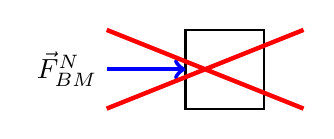
\begin{tikzpicture}
				\FBDbox{0,0}{0}{box}{}
				\draw[ultra thick,blue,->] (-1.5,0) -- (boxlcent);
				\node[anchor=east] at (-1.5,0) {$\vec{F}^{N}_{BM}$};
				\draw[ultra thick, red] (-1.5,0.5) -- (1,-0.5) (-1.5,-0.5) -- (1,0.5);
			\end{tikzpicture}
		\end{center}
		\item We also don't want the arrow to overlap the interior of the box. We will do something like this when we get to rigid-body diagrams in PH 212, but for now, it is better to keep the arrows pointed away for clarity.
		\begin{center}
			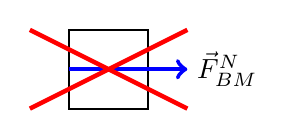
\begin{tikzpicture}
				\FBDbox{0,0}{0}{box}{}
				\FBDvectorXY{boxlcent}{1.5,0}{}
				\node[anchor=west] at (tip) {$\vec{F}^{N}_{BM}$};
				\draw[ultra thick, red] (-1,0.5) -- (1,-0.5) (-1,-0.5) -- (1,0.5);
			\end{tikzpicture}
		\end{center}
	\end{itemize}
\end{itemize}
\end{TeacherMargin}
\begin{PresentSpace}
\vspace{-10pt}
\section*{L8-1: Moving a Box}
\vspace{100pt}
Mike and Lucas are attempting to move a box, which does not move.
\begin{itemize}
	\item Identify all forces acting on the box.
	\item Draw a free-body diagram for the box.
	\item Indicate the acceleration.
\end{itemize}
\end{PresentSpace}
\begin{textblock*}{5cm}(14cm,1.75cm)
\centering
\includegraphics[scale=1.5]{Mike_and_Lucas_Fruitlessly_Push_a_Box.pdf}
\end{textblock*}
\newpage
\begin{TeacherMargin}
\noindent\textbf{Idenfity All Forces}
\begin{itemize}
	\item We still have most of the old forces: $\vec{F}^{N}_{BM},\ \vec{F}^{g}_{BE},\ \vec{F}^{T}_{BR},\ \vec{F}^{N}_{BG}$.
	\item The box is sliding, so we have kinetic friction instead of static: $\vec{F}^{kf}_{BG}$.
	\item We need to add the psychic force exerted on the box by Eleven: $\vec{F}^{ps}_{B11}$.
	\item The box is sitting on the ground and not budging, so we need a normal force on the box from the ground, and a force of static friction on the box from the ground: $\vec{F}^{N}_{BG}$ and $\vec{F}^{sf}_{BG}$.
\end{itemize}
\noindent\textbf{Free-Body Diagram}
\vspace{-0.75cm}
\begin{center}
	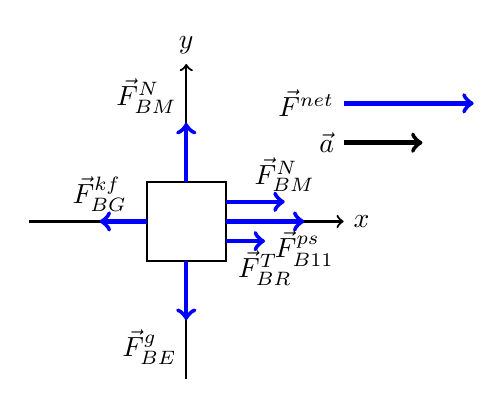
\begin{tikzpicture}
		\FBDaxes{0,0}{0}{axes}
		\FBDbox{axes}{0}{box}{}
		\FBDvectorXY{boxrtq}{0.75,0}{FNM}
		\node[anchor=south] at (FNMtip) {$\vec{F}^{N}_{BM}$};
		\FBDvectorXY{boxrbq}{0.5,0}{FTR}
		\node[anchor=north] at (FTRtip) {$\vec{F}^{T}_{BR}$};
		\FBDvectorXY{boxrcent}{1,0}{FP}
		\node[anchor=north] at (FPtip) {$\vec{F}^{ps}_{B11}$};
		\FBDvectorXY{boxlcent}{-0.6,0}{FKF}
		\node[anchor=south] at (FKFtip) {$\vec{F}^{kf}_{BG}$};
		\FBDvectorXY{boxtcent}{0,0.75}{FNG}
		\node[anchor=south east] at (FNGtip) {$\vec{F}^{N}_{BM}$};
		\FBDvectorXY{boxbcent}{0,-0.75}{FG}
		\node[anchor=north east] at (FGtip) {$\vec{F}^{g}_{BE}$};
		\node[anchor=east] at (2,1.5) {$\vec{F}^{net}$};
		\FBDvectorXY{2,1.5}{1.65,0}{Fnet}
		\node[anchor=east] (ACCEL) at (2,1) {$\vec{a}$};
		\draw[ultra thick,->] (ACCEL) -- (3,1);
	\end{tikzpicture}
\end{center}
\vspace{-0.75cm}
\textbf{Notes}
\begin{itemize}
	\item Kinetic friction is weaker than static friction; it is harder to start an object sliding than to keep it sliding.
	\item $\vec{F}^{net}$ is nonzero, as the horizontal forces are no longer balanced.
\end{itemize}
\textbf{Symbolic Expression} \\
The net force is the \textbf{vector} sum of all forces on the object. Each $\vec{F}$ contains direction information, so you should not put in minus signs at this point:
\[
\vec{F}^{net} = \vec{F}^{N}_{BG} + \vec{F}^{N}_{BM} + \vec{F}^{T}_{BR} + \vec{F}^{ps}_{B11} + \vec{F}^{g}_{BE} + \vec{F}^{kf}_{BG}.
\]
The components of a force are scalars \textbf{with signs}, so they also contain direction information specific to their particular coordinate axes. There is no need to add minus signs when breaking Newton's 2nd law into components. At this stage, it is appropriate to drop components that you know to be zero:
\begin{align*}
	F^{net}_{x} & = F^{N}_{BM,x} + F^{T}_{BR,x} + F^{ps}_{B11,x} + F^{kf}_{BG,x}, \\
	F^{net}_{y} & = F^{N}_{BG,y} + F^{g}_{BE,y}.
\end{align*}
When I write the components in terms of the magnitudes of the vectors, I have to add signs, as magnitudes are always positive. In particular, $F^{kf}_{BG,x} = -F^{kf}_{BG}$, and $F^{g}_{BE,y} = -F^{g}_{BE}$. We also know that the box slides horizontally, so $a_{y}=0$:
\begin{align*}
	ma_{x} = F^{net}_{x} & = F^{N}_{BM} + F^{T}_{BR} + F^{ps}_{B11} - F^{kf}_{BG}, \\
	0 = ma_{y} = F^{net}_{y} & = F^{N}_{BG} - F^{g}_{BE}.
\end{align*}
Therefore
\[
a_{x} = \frac{F^{N}_{BM} + F^{T}_{BR} + F^{ps}_{B11}-F^{kf}_{BG}}{m}.
\]
\end{TeacherMargin}
\begin{PresentSpace}
\vspace{-10pt}
\section*{L8-2: Moving a Box II}
\vspace{100pt}
El pushes the box with her mind, and it begins to speed up.
\begin{itemize}
	\item Modify your free-body diagram.
	\item Indicate the acceleration.
	\item Write a symbolic expression for the acceleration.
\end{itemize}
\end{PresentSpace}
\begin{textblock*}{5cm}(12.5cm,1.75cm)
\centering
\includegraphics[scale=1.5]{Eleven_Helps_Mike_and_Lucas_Push_a_Box.pdf}
\end{textblock*}
\newpage
\begin{TeacherMargin}
	
\end{TeacherMargin}
\begin{PresentSpace}
\section*{Main Ideas}
\begin{itemize}
	\item Forces arise from interactions between objects.
	\item There are many different kinds of forces that we can analyze differently.
	\item Objects can only change their motion when acted upon by an external force.
	\item The net force on an object is equal to its mass times its acceleration.
\end{itemize}
\end{PresentSpace}
\end{document}